%!TEX root = ../template.tex %
% !TeX spellcheck = en_US
%%%%%%%%%%%%%%%%%%%%%%%%%%%%%%%%%%%%%%%%%%%%%%%%%%%%%%%%%%%%%%%%%%%%
%% chapter4.tex
%% NOVA thesis document file
%%
%% Chapter with lots of dummy text
%%%%%%%%%%%%%%%%%%%%%%%%%%%%%%%%%%%%%%%%%%%%%%%%%%%%%%%%%%%%%%%%%%%%

\typeout{NT FILE chapter6.tex}%

\chapter{Electrostatic Screening in Two-dimensional materials}
\label{ch:screening}

In the intro of the chapter I can introduce the materials studied, revisiting hBN, and introduce \textbf{MoS2}.
Talk about band structure and a bit of the \abinit~methods used (CRYSTAL and Wannierization).

\textcolor{blue}{The following paragraph is in blue, to highlight that it was taken from the notes ipsis verbis. I believe it can be adapted to be included in the intro of the chapter.}

\textcolor{blue}{We have not hitherto specified the form of the Coulomb potential, even though screening was the main focus of the previous sections.
But it is well-known in the literature, that when dealing with pair-wise particle interactions, screening has to be taken into account~\cite{Latini_2015,Cudazzo_2011}. \textcolor{blue}{(Ignoring screening is actually one of the pit-falls of the \hf~ method.)}
This is why we had to develop a framework to incorporate it.
The first version of the code~\cite{Xatu} accounted for screening by using a linear model, the Rytova-Keldysh potential, that we have already introduced in the previous section.
Other works using RK: \cite{Dias_Silveira_Qu_2023,PhysRevB.98.125308}
In the intro I can also say that screening is important as shown by Latini and Thygesen~\cite{Latini_2015}...
Even though it works for a certain class of 2D semiconductors and insulators, such as monolayer \hbn, a further look into its form reveals that taking the $q \to 0$ limit in the static dielectric function leads to unphysical behaviours.
For instance, the Rytova-Keldysh dielectric function obtained taking into account the layer thickness of the active material and the dielectric environment, it might happen that the linearized model has a negative slope~\cite{Trolle_Pedersen_Veniard_2017}.
Furthermore, if we take the limit $q \to \infty$, then the screened potential  scales as $\sim 1/q^2$, whose (2D) inverse Fourier transform does scale with $\sim 1/r$.
Here we make the extension of the code to go beyond the Rytova-Keldysh approximation to compute the interaction matrix elements to build the Bethe-Salpeter Hamiltonian and solve the Bethe-Salpeter equation.}

\textcolor{red}{Explain that a strict 2D approach to screening has been done before with good results in analytical calculations for ungapped materials, e.g. graphene \cite{Hwang_2007,Sohier_Calandra_Mauri_2015}, and for numerical ones applied to excitons in 2D materials~\cite{Xatu,Cudazzo_2011,Ninhos_Tserkezis_Mortensen_Peres_2024,Henriques_Amorim_Ribeiro_Peres_2022,Henriques_Epstein_Peres_2022,Henriques_Peres_2020,Thygesen_2017}.}

One more abinit work: \cite{Prandini_Galante_Marzari_Umari_2019}

\section{Dielectric Function Revisited: Theory}
\label{sec:dielectric_function_revisited}

%Here we recall the expression of the microscopic dielectric function in 2D, and take it for insulators and semiconductors and the static limit.

In this section we look again into the \rpa~dielectric function we have previously introduced in Section~\ref{subsec:rpa_dielectric_function}.
The dielectric function in real-space and time domain, within \rpa, that we discussed in Section~\ref{sec:dielectric_function_quantum} writes

\begin{equation}
\label{eq:dielectric_function_real_time_recalled}
    \varepsilon (\br,\br';t,t') = \delta(\br - \br') \delta(t-t') - \int  v_c(\br - \br'') \chi^0 (\br'',\br';t-t') \dr''  \,,
\end{equation}

\noindent where $v_c$ denotes the bare (without screening) Coulomb potential and $\chi^0$ is the \rpa~irreducible polarizability.
When Fourier transformed from the $(\br,t)$ domain to the $(\omega,\bq)$ domain, it has the form

\begin{equation}
    \label{eq:dielectric_function_momentum_frequency_repeated}
    \varepsilon_{\bG \bG'} (\bq,\omega) = \delta_{\bG \bG'} - v_c(\bq + \bG) \chi^0_{\bG \bG'} (\bq,\omega) \,,
\end{equation}

\noindent where $\bG$ and $\bG'$ are reciprocal lattice vectors, $\bq$ is a vector in the first \bz, and $\omega$ is the frequency.
This is nothing more than a recapitulation of what we have discussed in Section~\ref{sec:dielectric_function_quantum}.
The novelty in this chapter is that the Fourier transform is not in three dimensions, but in two dimensions while overlooking the $z$ dimension, as if $\br=(x,y)$.
Since in this work we deal with \bd~materials, we argue that performing a \bd~Fourier transform on the dielectric function is the right thing to do, because the material is infinite in the $xy$ plane, but finite along the $z$-direction.
Technically speaking, we are saying that the response to an off-plane varying external potential is local, so that $\varepsilon(\br,\br') = \varepsilon^{\BD}(\br_{||},\br_{||}') \delta(z-z')$, where $\varepsilon^{\BD}$ is a strictly \bd~dielectric function, where $\br_{||}$ and $\br_{||}'$ are in-plane vectors, whose Fourier transform is~\eqref{eq:dielectric_function_momentum_frequency_repeated}.

Within the strict \bd~framework for the dielectric response we develop here, we can ignore the $z$ coordinate altogether in the dielectric function.
This is evidently an approximation that needs to be justified.
We postpone doing so to Section~\ref{subsec:quasi_2D}, and let us see how far we can go with a pure \bd~picture.
In what follows, we drop the $\BD$ superscript in $\varepsilon$ for ease of notation.
But still, the reader should keep in mind that it is a \bd~quantity.

In what follows all the geometric quantities like position, reciprocal lattice vectors, and momentum are in-plane.
Therefore, the momentum-resolved Coulomb potential in Eq.~\eqref{eq:dielectric_function_momentum_frequency_repeated} reads
\todo[inline]{Shorten the white space after writing the intro.}
\begin{equation}
    \label{eq:coulomb_momentum_repeated}
    v_c(\bq) =  \frac{e}{2  \epsz q} \,,
\end{equation}

\noindent which depends on momentum as $~1/q$, unlike its \gls{3d} counterpart that goes with $~1/q^2$.
As we will explain in a moment, this small detail puts us in advantage over typical first-principle approaches.

Naturally, the polarizability $\chi^0_{\bG \bG'} (\bq,\omega)$ is also the \bd~counterpart of Eq.~\eqref{eq:polarizability_momentum_frequency}, and reads

\begin{equation}
\label{eq:2D_polarizability}
    \chi^0_{\bG \bG'} (\bq,\omega) = \frac{1}{\area} \sum_{n,n'} \sum_{\bk \sigma} (f_{n,\bk} - f_{n',\bk + \bq}) \frac{\mel{n,\bk}{\ee^{-\ii(\bq + \bG) \vdot \br}}{n',\bk + \bq} \mel{n',\bk + \bq}{\ee^{\ii(\bq + \bG') \vdot \br}}{n,\bk}}{\epsilon_{n \bk} - \epsilon_{n' \bk + \bq} + \hw + \ii \hbar \alpha}\,.
\end{equation}

\noindent At the end, the expressions~\eqref{eq:dielectric_function_momentum_frequency_repeated} and~\eqref{eq:2D_polarizability} do not differ by much.
Their similarities are apparent from their written forms, but they greatly contrast in their implementation.
First of all, the sum over momentum $\bk$ is a sum over the \bd~\bz~of the material.
Furthermore, even though it is not explicitly evidentiated in the braket notation, the plane-wave matrix elements in the numerator amount to real-space integrals extending over the plane of the material, and are therefore integrals in \bd~space.
Such matrix elements have appeared before in Section~\ref{subsec:interaction_matrix_elements_and_screening}, when discussing the interaction matrix elements for the \bse~within an exact diagonalization formalism.
To make this chapter as self-contained as possible, we repeat the definition in Eq.~\eqref{eq:plane_wave_matrix_element_definition} from that section, but now making it explicit that the integral is in two dimensions.
Henceforth, we can write

\begin{equation}
\label{eq:2D_plane_wave_matrix_element}
    I^{\bG}_{n \bk, n' \bk'} \equiv \bra{n,\bk} \ee^{-\ii (\bk - \bk' + \bG) \vdot \br} \ket{n',\bk'} = \int_{\area} \dr\, \psi^*_{n,\bk} (\br) \ee^{-\ii(\bk  - \bk' + \bG) \vdot \br} \psi_{n', \bk'} (\br)\,.
\end{equation}

\noindent Note that even though the notation is similar to that of Ref.~\cite{Xatu}, the definition for $I^{\bG}_{n \bk, n' \bk'}$ is not exactly the same.
We will explain how to compute the matrix elements and the polarizability in practice in the next subsection.

\subsection{Noninteracting polarizability}
\label{subsec:non_interacting_polarizability}

Since we are interested in electrostatic screening for \bd~insulators and semiconductors (from now on, let us just say insulators to account for all \bd~gapped materials), and at very low temperatures, we can simplify the polarizability in Eq.~\eqref{eq:2D_polarizability} to

\begin{equation}
    \label{eq:static_polarizability_repeated}
    \begin{aligned}
        \chi^0_{\bG\bG'}(\bq,\omega \to 0) = & \frac{1}{\area} \sum_{\vv \cc,\bk \sigma} \Bigg[\frac{\langle \cc,\bk| \ee^{-\ii(\bq+\bG)\cdot\br}|\vv,\bk+\bq\rangle \langle \vv,\bk+\bq| \ee^{\ii(\bq+\bG')\cdot\br}|\cc,\bk\rangle}{\epsilon_{\vv \bk+\bq}-\epsilon_{\cc \bk}} \Bigg] + \\
        & \frac{1}{\area} \sum_{\vv \cc,\bk \sigma} \Bigg[\frac{\langle \vv,\bk| \ee^{-\ii(\bq+\bG)\cdot\br}|\cc,\bk+\bq\rangle\langle \cc,\bk+\bq| \ee^{\ii(\bq+\bG')\cdot\br}|\vv,\bk\rangle}{\epsilon_{\vv \bk} - \epsilon_{\cc \bk+\bq}}\Bigg] \,,
    \end{aligned}
\end{equation}

\noindent where the sum over bands $n$ and $n'$ is now over valence bands $\vv$ and conduction bands $\cc$.
In the previous expression, if the system enjoys \gls{trs}, then the two terms on the right-hand side add up so that we can write the polarizability in a more compact form as

\begin{equation}
    \label{eq:static_polarizability_TRS}
    \chi^0_{\bG \bG'} (\bq) = \frac{2}{\area} \sum_{\vv \cc}  \sum_{\bk \sigma} \frac{I^{\bG}_{\cc \bk, \vv \bk + \bq}  \qty(I^{\bG'}_{\cc \bk, \vv \bk + \bq})^*}{\epsilon_{\vv \bk + \bq} - \epsilon_{\cc \bk} }\,
\end{equation}

\noindent We would like to take this opportunity to make a brief remark.
We have confirmed analytically that expression~\eqref{eq:static_polarizability_repeated} derives from its more general version in~\eqref{eq:2D_polarizability}, which is an expression commonly found in textbooks~\cite{Cohen_Louie_2016}.
However, the expression in~\eqref{eq:static_polarizability_TRS} is not commonly found in textbooks, but it has made its appearance in the literature~\cite{BerkeleyGW,Yambo_2009}.
We stress that the prefactor of $2$ and the sum over spins $\sigma$ are key to correctly obtain the screening properties.
We prove in Appendix~\ref{app:polarizability_TRS_proof} that expression~\eqref{eq:static_polarizability_repeated} reduces to~\eqref{eq:static_polarizability_TRS} when \gls{trs} is present.
All systems considered in this thesis enjoy \gls{trs}, which can be broken, for instance, when a static magnetic field is applied.
As we have stated before in Section~\ref{subsec:maxwell_equations}, we do not study magnetized media.

We have gathered all the necessary knowledge to compute these matrix elements, and thus the matrix elements of the noninteracting polarizability $\chi^0_{\bG \bG'}(\bq)$.
As we said before, the material is in practice \bd~without any repeated off-plane images, unlike in first-principle approaches.
Therefore, our implementation is strictly \bd, and we ignore, for the moment, any information pertaining to the out-of-plane degrees of freedom.
This means that:

\begin{itemize}
    \item The sum over momentum in~\eqref{eq:static_polarizability_repeated} is a sum over momentum $\bk = (k_x,k_y)$ in the \bz, which is \bd.
    \item The $\bG$ and $\bG'$ vectors are \bd~vectors of the reciprocal lattice, which is \bd.
    \item The matrix element $I^{\bG}_{n \bk, n' \bk'}$ that is an integral in real space when written in terms of Bloch state wavefunctions, is an integral in the $xy$ plane. The symbol $\dr$ inside the integrals therefore means $\dd x \dd y$, if we do not say otherwise.
\end{itemize}

\noindent With this information in mind, we can work out the plane-wave matrix elements by replacing the Bloch wavefunctions by their expression in terms of localized orbitals, that in the lattice gauge read

\begin{equation}
    \label{eq:Bloch_state_LCAO_repeated}
    \psi_{n \bk} (\br) = \frac{1}{\sqrt{N}} \sum_{\bR} \ei{\bk \vdot \bR} \sum_{i \alpha} C_{i \alpha}^{n \bk} \phi_{\alpha} (\br - \bR - \bt_i)\,.
\end{equation}

\noindent The plane-wave matrix elements between Bloch states have actually been calculated before in Section~\ref{sec:bethe_salpeter_equation_effective_models}, at the time when we derived the \bse~applied to effective models.
At this stage, we compute them approximately using once again the point-like orbital approximation, but beyond the envelope function approximation as we did in Section~\ref{sec:bethe_salpeter_equation_effective_models}.
Let us then carry out the integral once more.
We have

\begin{align}
    \label{eq:lane_wave_matrix_element}
    I^{\bG}_{n \bk, n' \bk'} =& \int \dr\, \psi^*_{n,\bk} (\br)\, \ee^{-\ii(\bk' - \bk + \bG) \vdot \br} \psi_{n' \bk'} (\br) = \notag \\
    =& \frac{1}{N} \int \dr \sum_{\bR \bR'} \ee^{- \ii \bk \vdot \bR} \ei{\bk' \vdot \bR'} \sum_{i \alpha j \beta} (C_{i \alpha}^{n \bk})^* C_{j \beta}^{n' \bk'} \underbrace{\phi^*_{\alpha} (\br - \bR - \bt_i) \phi_{\beta} (\br - \bR' - \bt_j)}_{\approx \delta_{ij} \delta_{\alpha \beta} \delta_{\bR \bR'} \delta(\br - \bR - \bt_i)} \ee^{-\ii(\bk' - \bk + \bG) \vdot \br} = \notag \\
    =& \frac{1}{N} \sum_{\bR} \cancel{\ee^{-\ii (\bk - \bk') \vdot \bR}} \sum_{i \alpha} (C_{i \alpha}^{n \bk})^* C_{i \alpha}^{n' \bk} \cancel{\ee^{-\ii (\bk' - \bk) \vdot \bR}} \ee^{- \ii \bG \vdot \bR} \ee^{- \ii (\bk' - \bk)  \vdot \bt_i} \ee^{-\ii \bG  \vdot \bt_i} =  \notag \\
    =& \frac{1}{N} \left(\sum_{\bR} \ee^{-\ii \bG \vdot \bR} \right) \sum_{i \alpha} (C_{i \alpha}^{n \bk})^* C_{i \alpha}^{n' \bk'}  \ee^{-\ii (\bk' - \bk + \bG)  \vdot \bt_i} = \notag \\
    =& \sum_{i \alpha} (C_{i \alpha}^{n \bk})^* C_{i \alpha}^{n' \bk'}  \ee^{-\ii (\bk' - \bk + \bG)  \vdot \bt_i}\,, \qq{since} \sum_{\bR} \ee^{-\ii \bG \vdot \bR} = N \,,
\end{align}

\noindent where from the 2nd line to the 3rd line we did the point-like orbital approximation, and from the 4th line to the 5th line we used the fact that by definition $\ee^{-\ii \bG \vdot \bR} = 1$.

To summarize, to compute a single polarizability matrix element $\chi^0_{\bG \bG'} (\bq)$ we need:

\begin{itemize}
    \item The Bloch Hamiltonian $H(\bk)$ (regardless of the gauge) and to diagonalize it to obtain the band structure $\{\epsilon_{n \bk}\}$ in the set of points $\bk$ included in the sum and the eigenvectors $\{\bC^{n \bk}\}$ storing the tight-binding coefficients $C^{n \bk}_{i \alpha}$;
    \item The set of energies $\{\epsilon_{n \bk + \bq} \}$ and eigenvectors $\{\bC^{n \bk + \bq}\}$, where $\bq$ is the point in the \bz~we are computing the polarizability at;
    \item The plane-wave matrix elements of the form $I^{\bG}_{\cc \bk, v \bk + \bq} = \sum_{i \alpha} (C_{i \alpha}^{c \bk})^* C_{i \alpha}^{v \bk + \bq}  \ee^{-\ii (\bq + \bG)  \vdot \bt_i}$, as we know the position of the atoms in the motif $\bt_i$ from the beginning.
\end{itemize}

In our numerical framework, the Bloch Hamiltonian $H(\bk)$ is determined by the input model for the code.
The code accepts two types of input.
One way is by providing an output file from CRYSTAL~\cite{CRYSTAL_23}, which contains the Fock matrices $H(\bR)$ which help defining the Bloch Hamiltonian through Eq.~\eqref{eq:Bloch_Hamiltonian_definition}, as we saw in Chapter~\ref{ch:quantum_mechanics_solids}.
Alternatively, the code accepts also \texttt{.model} files containing a tight-binding model for the material at hand.
Quite recently, the code was updated by G.~Janone with an utility that transforms an output file from Wannier90~\cite{Wannier90} into a \texttt{.model} file.
The corresponding version of the code can be found in \url{https://github.com/GuiJanone/xatu-w90}.
This utility serves as an intermediary between Wannier90 and the Xatu code.

The Wannier model for the Hamiltonian has to be obtained through the method of maximally localized Wannier functions~\cite{Marzari_2012}, in order for the point-like orbital approximation to be as true as possible.
Then, the orbitals $\phi_{\alpha}$ can be perceived as Wannier functions (see footnote~\ref{fn:Wannier_functions} in Chapter~\ref{ch:quantum_mechanics_solids}) as well, besides their interpretation as atomic orbitals.
In general, in a Wannier representation of the Hamiltonian, we have as many ``atomic positions'' $\bt_i$ as orbitals in total, but only one orbital per site within the motif of the unit cell.
On the contrary, in a tight-binding model, we have as many atomic positions $\bt_i$ as atoms in the motif, and generically more than one orbital per atom.
Either way, we do not consider the spatial structure of the orbitals, therefore our approach applies equally to both cases.
Upon diagonalization of the Bloch Hamiltonian $H(\bk)$ at momenta $\bk$ and $\bk + \bq$, we obtain the band structure from the eigenvalues and the tight-binding coefficients from the eigenvectors.
Using this information to compute the polarizability matrix elements, we can compute the elements of the dielectric function, which is the subject of the next subsection.

\subsection{Dielectric matrix and its inversion}
\label{subsec:dielectric_matrix_inverse}

We are interested in the static limit of the dielectric function as per Eq.~\eqref{eq:dielectric_function_momentum_frequency_repeated}, for which we need the static polarizability worked out in the previous section.
The static dielectric function, within \rpa, writes

\begin{empheq}[innerbox=\colorbox{lightgray}, right={\,,}]{align}
    \label{eq:static_symmetrized_dielectric_function}
    \varepsilon_{\bG \bG'} (\bq) = \delta_{\bG \bG'} - \sqrt{v_c(\bq + \bG)} \chi^0_{\bG \bG'} (\bq) \sqrt{v_c(\bq + \bG')}
\end{empheq}

\noindent if we adopt the symmetrized version of~\eqref{eq:dielectric_function_momentum_frequency_repeated}.
The reason why we implement the symmetrized version is that it eases the treatment of numerical divergences in the dielectric function and, subsequently, in the screened potential in the long-wavelength limit~\cite{Baldereschi_Tosatti_1978,Rasmussen_Schmidt_Winther_Thygesen_2016,Shishkin_Kresse_2006}.
Actually, for the head element $\varepsilon_{\bzero \bzero} (\bq \to \bzero)$, it is indifferent if we use the symmetrized version as per Eq.~\eqref{eq:static_symmetrized_dielectric_function}, or the initial one in Eq.~\eqref{eq:dielectric_function_momentum_frequency_repeated}.
For this element, we can simply set $\varepsilon_{\bzero \bzero} (\bq \to \bzero) = 1$, because the bare potential goes with $v_c(\bq) \sim 1/q$, while the polarizability goes with $\chi^0_{\bzero \bzero} (\bq \to \bzero) \sim q^2$, as we shall confirm in Subsection~\ref{subsec:non_interacting_polarizability_results}.
This feature of the head element of the polarizability is universal among insulators, either in two or three dimensions, as long as the material presents a bandgap~\cite{Thygesen_2017}.
This means that, when computing the matrix element $\varepsilon_{\bzero \bzero} (\bq)$ in the limit $\bq \to \bzero$, we face no numerical instabilities unlike in the \gls{3d} case, where $v_c(\bq) \sim 1/q^2$.

In \abinit~calculations for \bd~materials, it is typical to use a truncated Coulomb potential instead of the full one, in order to mitigate the interaction between repeated images, with increasing off-plane separation~\cite{Ismail-Beigi_2006,Huser_Olsen_Thygesen_2013,Rasmussen_Schmidt_Winther_Thygesen_2016}.
Only after performing a \bd~Fourier transform of the truncated Coulomb potential, and taking the limit $q \to 0$, one can obtain a $1/q$ behavior for the potential, removing any numerical instabilities when taking that limit.
However, it still depends on the off-plane separation between layers, $L_{\perp}$.
But even in that case, the value of the static macroscopic dielectric function, $\varepsilon_M$, at zero momentum is not exactly the unity~\cite{Huser_Olsen_Thygesen_2013}.
The results have to be converged by increasing $L_{\perp}$, and only in the limit of infinite separation $\varepsilon_M (0) = 1$ for a \bd~material.
Besides that, the \bd~macroscopic dielectric function is not simply the one given be the definition in Eq.~\eqref{eq:macroscopic_dielectric_function_definition}.
It is obtained only after performing an off-plane average of the inverse \gls{3d} microscopic dielectric function~\cite{Huser_Olsen_Thygesen_2013,Jornada_PhD,Diana_PhD}, as the definition in Eq.~\eqref{eq:macroscopic_dielectric_function_definition} is not directly applicable.

With our framework, the macroscopic dielectric function we get from inverting the microscopic one as per Eq.~\eqref{eq:static_symmetrized_dielectric_function} is automatically an effective \bd~macroscopic dielectric function.
Also, we have $\varepsilon_{\bzero \bzero} (\bzero) = \varepsilon^{-1}_{\bzero \bzero} (\bzero) = 1$ by construction.
Regarding the numerical treatment of the wing terms $\varepsilon_{\bzero \bG'} (\bq)$ and $\varepsilon_{\bG \bzero} (\bq)$, it is required to look at the asymptotic behaviour of the matrix elements of the dielectric matrix and its inverse when $\bq \to \bzero$.
Only in that way can we know how to avoid divergences or undefined values for the screened potential.
This is critical for the computation of the excitons, due to how the screened Coulomb potential enters in the calculation of the interaction matrix elements (see Eqs.~\eqref{eq:interaction_matrix_element_direct_reciprocal} and~\eqref{eq:interaction_matrix_element_exchange_reciprocal}).
Issues of these kind are routine in the literature~\cite{BerkeleyGW,Louie_2000,Rasmussen_Schmidt_Winther_Thygesen_2016,Guandalini_Varsano_2023}.
In order to not break the flow of the text, we relegate the details to Appendix~\ref{app:regularization}.

%%%%%%%%%%%%%%%%%%%%%%%%%%%%%%%%%%%%%%%%%%%%%%
The calculations are also much more efficient due to the reduced dimensionality of our approach.
To compute the dielectric matrix and invert it, we have no off-plane contribution to the reciprocal lattice vectors, so the number of matrix elements to compute, at each point $\bq \in \BZ$, scales with $N^2$ instead of $N^3$, if $N$ is the number of cells of the reciprocal lattice along the directions of the two primitive vectors.
Then, in two dimensions the number of linear combinations is $N^2$, and in three dimensions it is $N^3$.

After having computed the dielectric matrix, we need to invert it.
This poses a difficulty in the problem: there are infinite reciprocal lattice vectors; therefore, we need to apply a cutoff $G_c$ for the vectors $\bG$ and truncate the dielectric matrix to invert it in practice.
Even if we have decided to follow the alternative approach for the \rpa~inverse dielectric function, given by~\cite{Dielectric_Genome}

\begin{equation}
    \label{eq:inverse_dielectric_function_alternative}
    \varepsilon^{-1}_{\bG \bG'} (\bq) = \delta_{\bG \bG'} + v_c(\bq + \bG) \chi^{\RPA}_{\bG \bG'} (\bq) \,,
\end{equation}

\noindent where $\chi^{\RPA}_{\bG \bG'} (\bq)$ is the reducible polarizability within \rpa, defined by the Dyson equation \eqref{eq:Dyson_equation_chi_RPA}.
In that same equation, all quantities when written in momentum space are infinite matrices as well, so we would need to apply a cutoff for the vectors $\bG$ either way.
This is in great contrast with the jellium model considered by H.~Bruus and K.~Flensberg in Ref~\cite{Bruus_Flensberg_2004}, where there is no underlying crystalline structure, and as a consequence, all quantities like the Coulomb potential, the polarizability and the dielectric function are simply scalars.
For now, let us assume that we can in principle compute the dielectric matrix and invert it without any problems.
In that way, the screened Coulomb potential writes

\begin{equation}
    \label{eq:screened_static_Coulomb_potential}
    W_{\bG \bG'} (\bq) =  \varepsilon^{-1}_{\bG \bG'} (\bq) v_c(\bq + \bG') \text{lololo}
\end{equation}

\noindent in the static approximation, which we have to justify.
Looking at the dynamical expression of the polarizability, we can see that the frequency dependence comes from the denominator as $\hbar \omega - (\epsilon_{n' \bk+\bq} - \epsilon_{n \bk})$.
If the band gap estimated by $ \epsilon_{n' \bp} - \epsilon_{n \bp}$ (assuming it is direct and located at the point $\bp$ in the \bz) is large enough when compared to the frequency, then we can approximate the screened Coulomb potential by its static limit, and discard an integration in frequency in the interaction matrix elements.

To finish the discussion, we revisit the interaction matrix elements in the \gls{bse} for the excitons with the numerical approach.
Their expressions derived in Section~\ref{subsec:interaction_matrix_elements_and_screening} remain the same.
Namely for the direct term we have

\begin{empheq}[innerbox=\fbox, right={\,,}]{align}
    \label{eq:direct_term}
    D_{\vv\cc,\vv'\cc'}(\bk,\bk',\bQ) = \frac{1}{N} \sum_{\bG,\bG'} \qty(I^{\bG}_{\cc \bk+\bQ, \cc' \bk'+\bQ})^* W_{\bG \bG'}(\bk - \bk') I^{\bG'}_{\vv \bk, \vv' \bk'}
\end{empheq}

\noindent and for the exchange term

\begin{empheq}[innerbox=\fbox,right={\,.}]{align}
    \label{eq:exchange_term}
    X_{\vv\cc,\vv'\cc'}(\bk,\bk',\bQ) = \frac{1}{N} \sum_{\bG,\bG'} \qty(I^{\bG}_{\cc \bk+\bQ, v \bk})^* W_{\bG \bG'}(\bQ) I^{\bG'}_{\cc' \bk' + \bQ, \vv' \bk'}
\end{empheq}

\noindent The reader shall notice that in both expressions there is a sum over reciprocal lattice vectors.
In fact, it is a double sum over $\bG$ and $\bG'$.
This double sum accounts for local-field effects in the calculation of the excitons, which derives from the translational invariance being discrete and not continuous.
If we have enough $(\bG,\bG')$ matrix elements in the dielectric function, in principle we will not need as many terms in the sums above.
In practice, we have two cutoffs, one for the dielectric function $G_c$, and another one for the excitons $G_{\cc,X}$.
To preserve basic symmetries and degeneracies, we hope that $G_{\cc,X}$ can be made small enough compared to $G_c$\footnote{In practice, we always have $G_{\cc,X} < G_c$, since we have to compute the dielectric matrix before computing the exciton.}.
We shall study that in our results in the next section.

\section{Dielectric Function Revisited: Numerical Results}
\label{sec:dielectric_function_results}

Here we analyze the numerical results obtained from the implementation of the theoretical concepts we have just described.
We will follow the same order as in the previous section; we focus first on the polarizability, then on the dielectric matrix and its inverse, and finally the excitons.
When discussing the dielectric function, we shall make the connection with the macroscopic dielectric function, and take the small-$\bq$ limit.
In principle, we are able to recover the Rytova--Keldysh model and get an estimate for the screening parameter $r_0$.
The material of choice is \gls{hbn} once more; but now, we work with a more realistic model as we shall describe.

\subsection{hBN revisited: DFT band structure and Hamiltonian model}
\label{subsec:hBN_revisited}

In this section we describe our model Hamiltonian for \gls{hbn}, a \bd~material quite important in this work.
We have seen before a minimal tight-binding model for \gls{hbn} in Section~\ref{subsubsec:tight_binding_method}, with only two parameters; the onsite energy difference between boron and nitrogen atoms, and the hopping parameter between first neighbor sites.
Then later on chapter~\ref{ch:Optical_hBN_superlattice}, we used a model based on the initial one considered in chapter~\ref{ch:quantum_mechanics_solids} to study excitons and the excitonic optical response in a \gls{hbn} nanostructure.
We also used the Rytova--keldysh model to account for the screening.
In this chapter, we work out a numerical model for \gls{hbn}, but for that, we need a more realistic model for that material using \abinit~methods.
After all, it is with \abinit~methods that we can obtain tight-binding parameters for different materials.

Herein, the model Hamiltonian for \gls{hbn} was obtained through \dft~calculations using the commercial package CRYSTAL~\cite{CRYSTAL_23}, which uses a basis of Gaussian functions.
The hybrid functional HSE06\todo{need a Ref maybe} was used with the Perdew--Burke--Ernzerhof functional~\cite{Perdew_1996} within the \gls{gga}, with a $48\times48\times1$ $k$-grid.
The output file $\texttt{hBN\_base\_HSE06.outp}$ extension can be found in the official repository for the Xatu code~\cite{Xatu}; \url{https://github.com/alejandrojuria/xatu}.
This file contains the Fock matrices of the form $H(\bR)$ in a basis of localized Gaussian functions, sufficient in number to build the Bloch Hamiltonian $H(\bk) = \sum_{\bR} \ee^{\ii \bk \cdot \bR} H(\bR)$.
If the reader needs to be reminded of these concepts, we refer to Section~\ref{subsubsec:tight_binding_method} of chapter~\ref{ch:quantum_mechanics_solids}.
Upon diagonalization of the Bloch Hamiltonian along the high-symmetry line $\Gamma-K-M-\Gamma$, we obtained the band structure displayed in Fig.~\ref{fig:hBN_DFT_bands} below.
With this model Hamiltonian, namely the band structure and the eigenvectors of the Bloch Hamiltonian, we construct a numerical model for the screening properties of \gls{hbn}, needed later on to compute the excitons through exact diagonalization of the \bse, in particular the interaction matrix elements, as discussed in Section~\ref{subsec:interaction_matrix_elements_and_screening}.
That is the subject of the sections to come.

\begin{figure}[H]
    \centering
    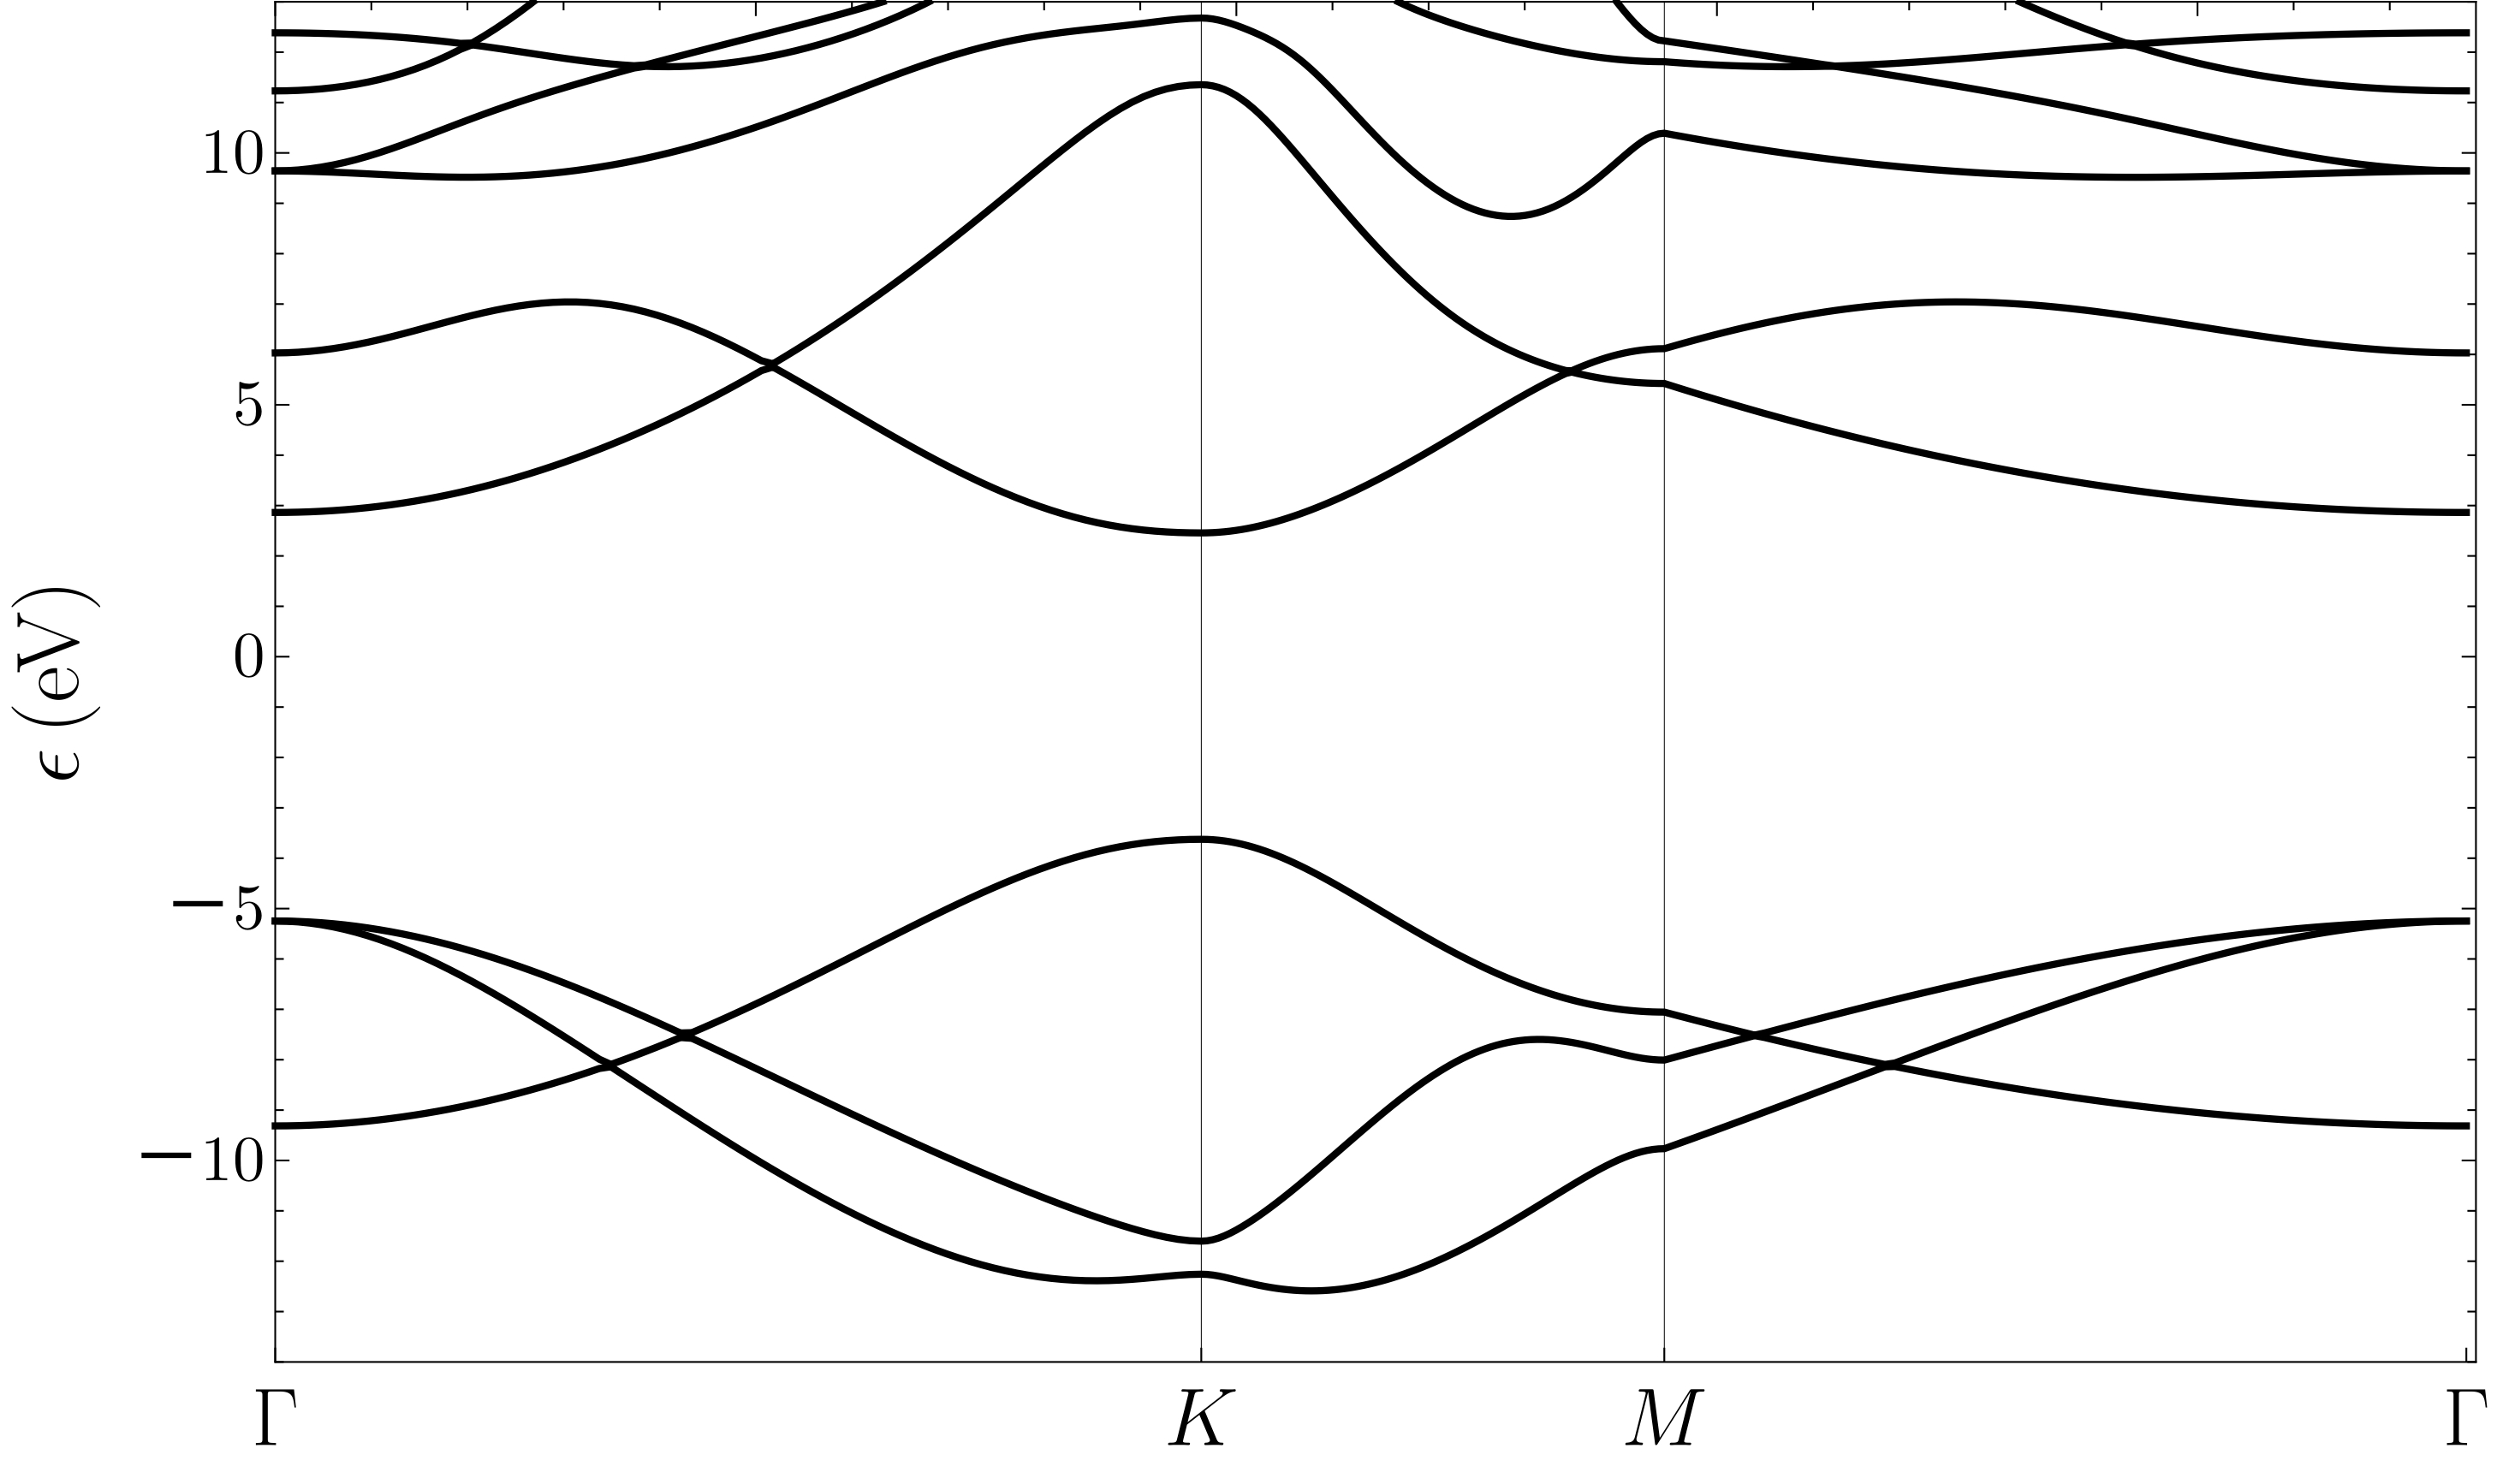
\includegraphics[width=0.9\linewidth]{Chapters/Figures/Chapter_6/hBN_HSE06_bands}
    \mycaption[Band structure of \gls{hbn} through first-principle methods]{Band structure of monolayer \gls{hbn} computed through first-principle methods, namely, within \dft~using the HSE06 functional as the exchange--correlation functional, with the CRYSTAL package.}
    \label{fig:hBN_DFT_bands}
\end{figure}

\subsection{Noninteracting polarizability}
\label{subsec:non_interacting_polarizability_results}

Before we proceed with the calculation of the dielectric matrix, we need to study the convergence of the matrix elements of the polarizability $\chi^0_{\bG \bG'} (\bq)$ given in Eq.~\eqref{eq:static_polarizability_TRS} with the number of included conduction bands, for different $(\bG,\bG')$ pairs, and for different values of momentum $\bq$.
\todo{Add a word on convergence with k-points.}

In Fig.~\ref{fig:chi_00_hbndft} below, we study the convergence of the polarizability with the number of empty bands included in the calculation for hBN, in particular the element $\chi^0_{\bzero \bzero} (\bq)$.
The $(\bG,\bG') = (\bzero,\bzero)$ matrix element is commonly called in the literature the head element.
In this example the band structure was obtained within \dft~with the HSE06 functional using CRYSTAL~\cite{CRYSTAL_23}, and 169 Fock matrices were included in the calculations.
We see again that the polarizability converges with the number of empty bands included.
In Fig.~\ref{fig:chi_g1_0_hbndft} we do a similar analysis to proof check that the polarizability converges as well when for different matrix elements other than the head.
We picked an off-diagonal element to check for convergence of both real and imaginary parts.
We can see that both real and imaginary parts of the chosen matrix element converge well with the number of conduction bands.
Something similar has been seen before in other works in the literature, such as Ref.~\cite{BerkeleyGW}, in figure 4 therein.

\begin{figure}[H]
    \centering
    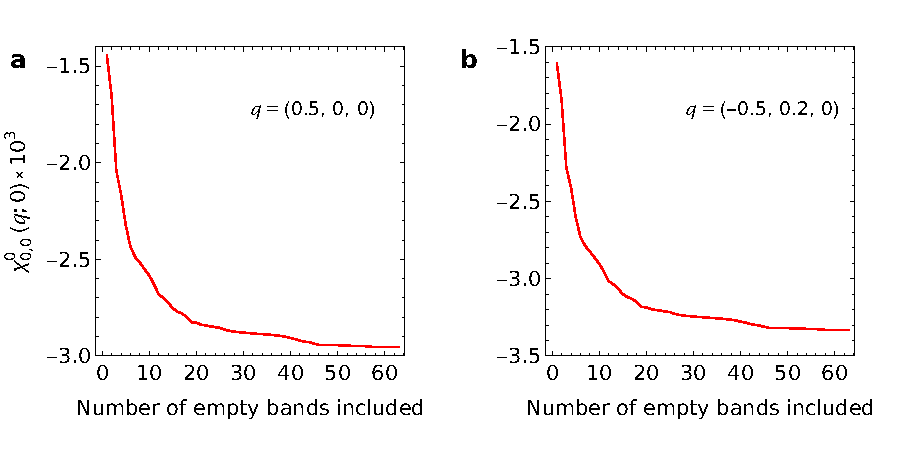
\includegraphics[width=0.9\linewidth]{Chapters/Figures/Chapter_6/Chi00hBNDFTq1&q2}
    \mycaption[Convergence of the polarizability with the number of conduction bands: head element]{Matrix element $\chi^0_{\bzero \bzero} (\bq)$ of the polarizability for two different values of momentum $\bq$ as a function of included conduction bands for hBN, whose bands were obtained within \dft~with the HSE06 functional using the CRYSTAL package.}
    \label{fig:chi_00_hbndft}
\end{figure}

\begin{figure}[H]
    \centering
    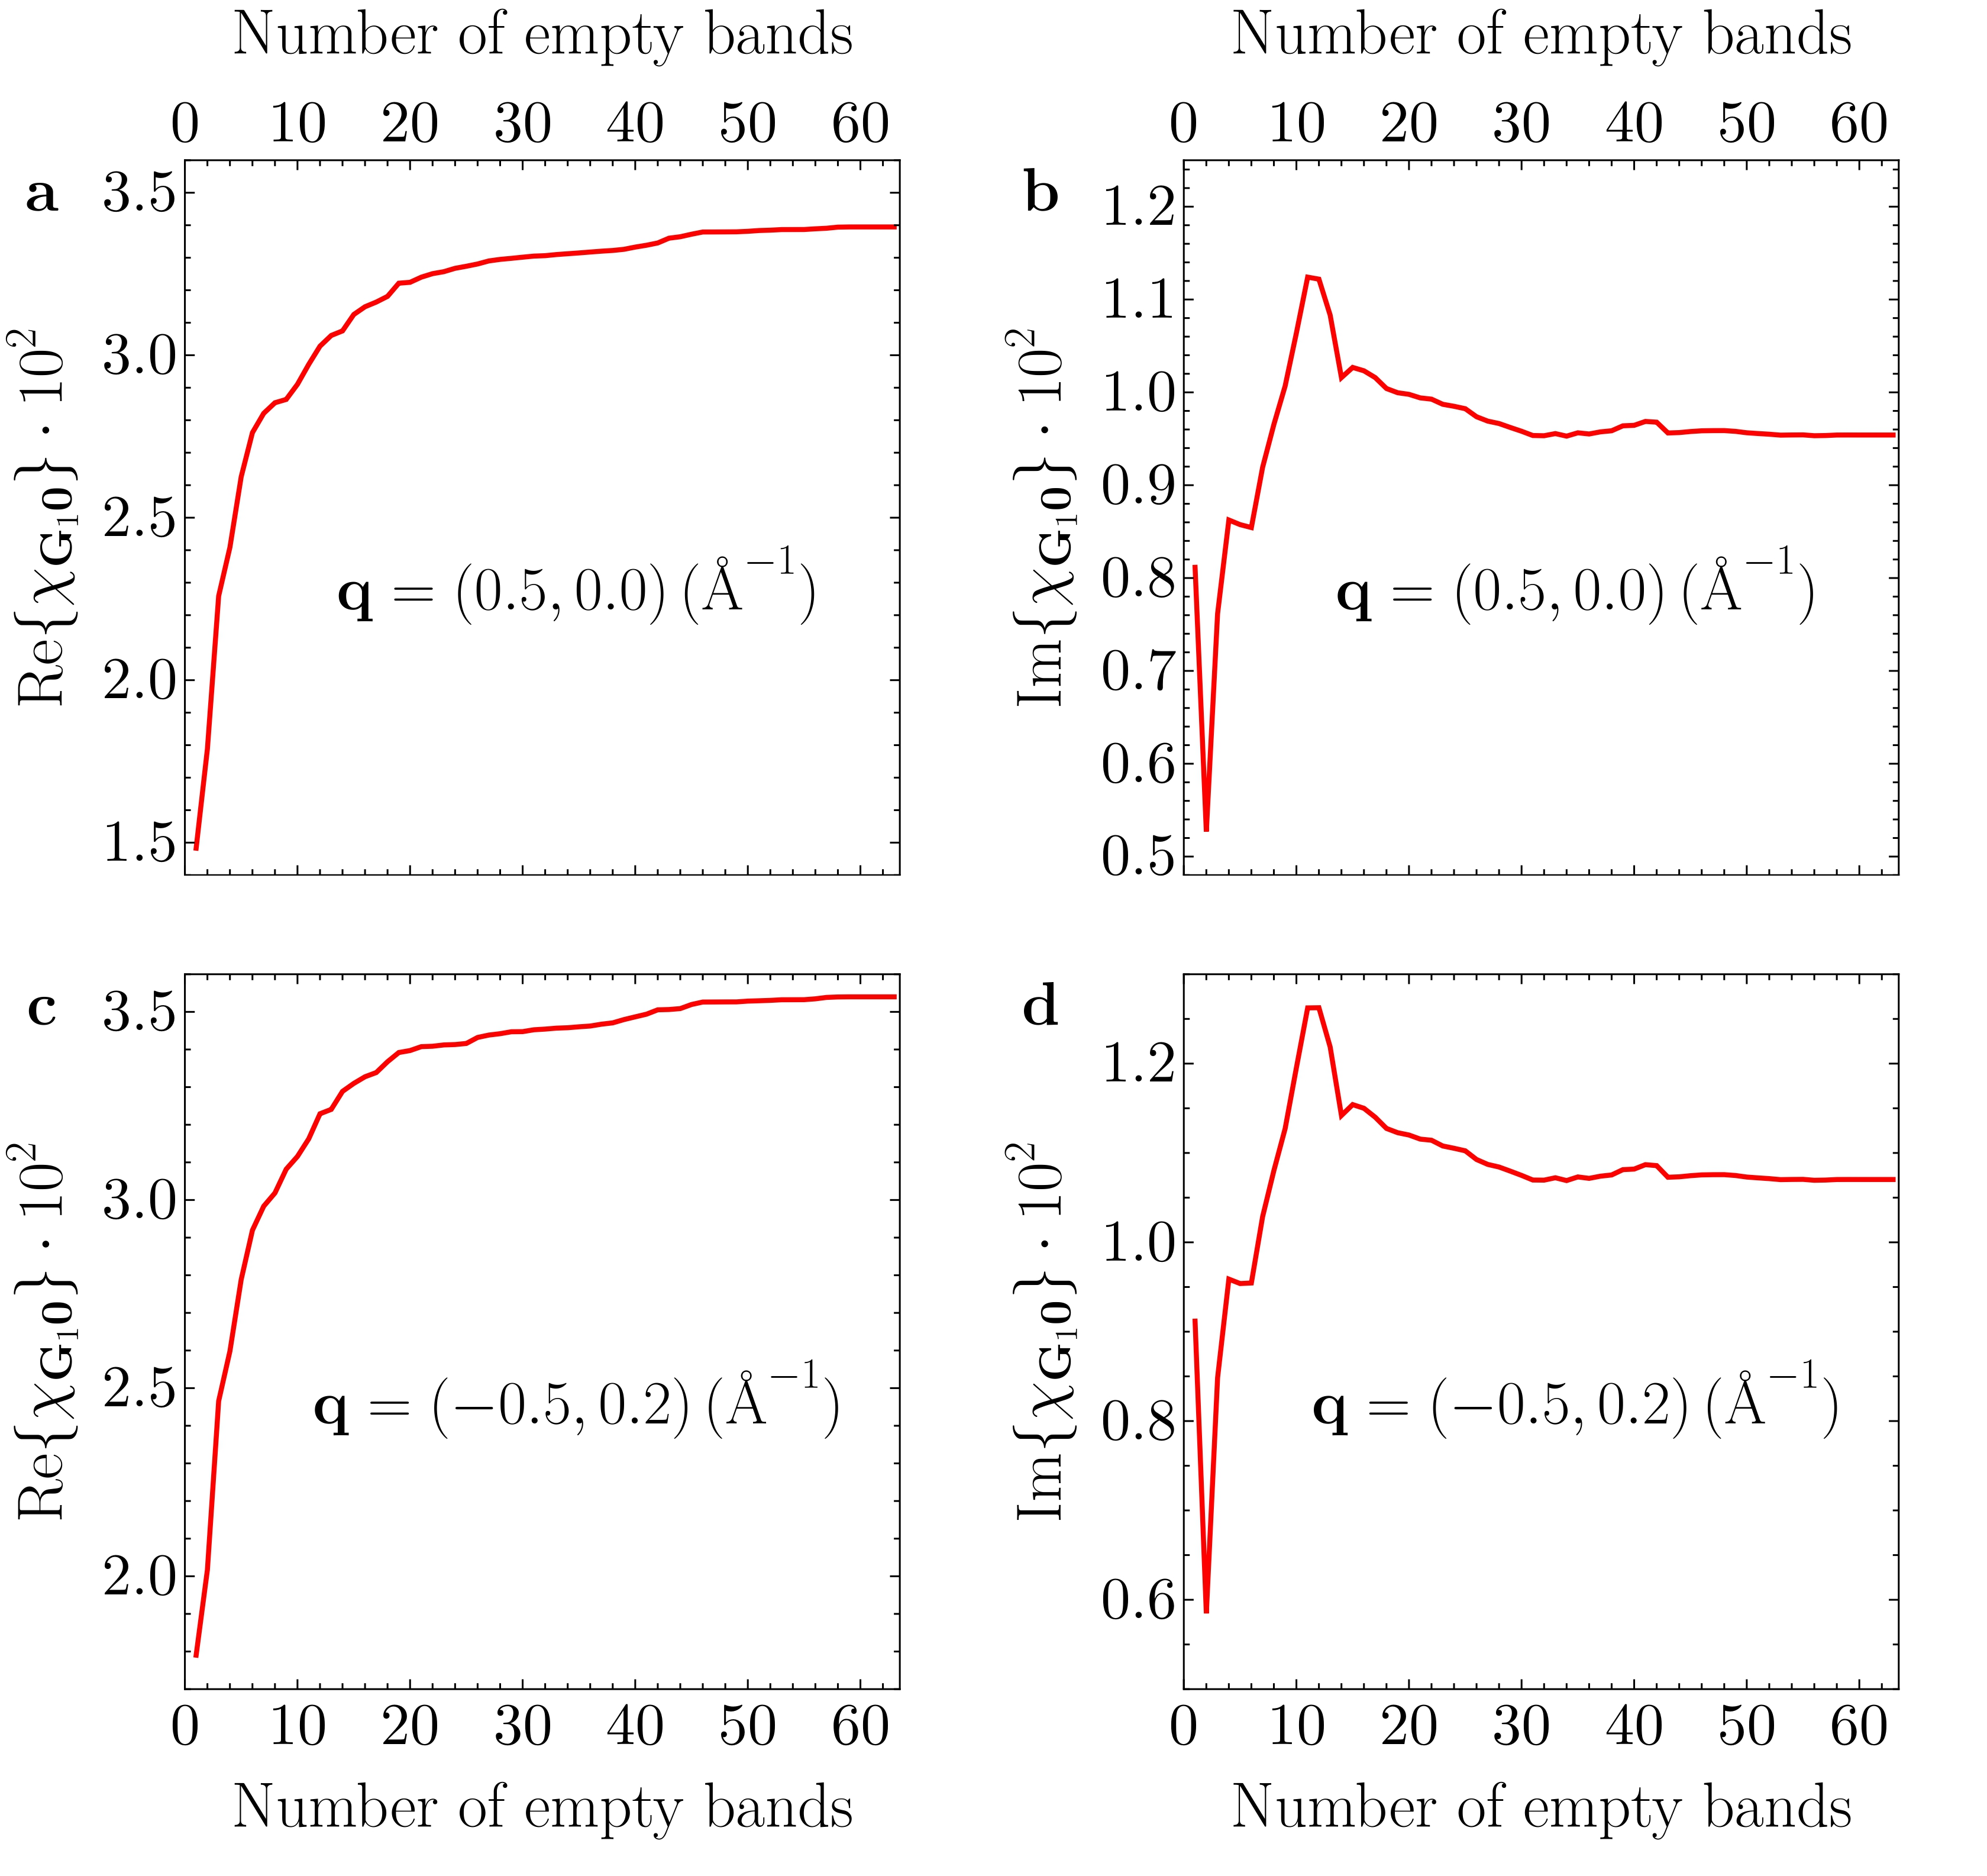
\includegraphics[width=0.9\linewidth]{Chapters/Figures/Chapter_6/ChiG1_0hBNDFTq1&q2}
    \mycaption[Convergence of the polarizability with the number of conduction bands: an off-diagonal]{Matrix element $\chi^0_{\bG_1 \bzero} (\bq)$ of the polarizability, where $\bG_1$ is the vector of the reciprocal lattice with the shortest length, for two different values of momentum $\bq$ as a function of included conduction bands for hBN. The left panels display the real part, while the right panels display the imaginary part. The model for hBN is the same as in Fig.~\ref{fig:chi_00_hbndft}.}
    \label{fig:chi_g1_0_hbndft}
\end{figure}

Next we study how the polarizability behaves for any momentum $\bq \in \BZ$.
We start with the head matrix element.
In Fig.~\ref{fig:chi_00_hbndft_mesh} below we plot the $\chi^0_{\bzero \bzero} (\bq)$ in the \bz~mesh, more precisely in panel \pnl{b}.
Panel \pnl{a} displays the quantity $\chi^0_{\bzero \bzero} (\abs{\bq})$ for two different directions for $\bq$, along the $q_x$ axis in dashed blue, and parallel to the reciprocal lattice vector parallel to the side of the parallelogram in purple stripes.
The red dots represent $\chi^0_{\bzero \bzero} (\bq)$ for all points $\bq$ in the mesh.
The purpose of these plots was to confirm that the computed polarizability for hBN is isotropic, as expected.
Out of curiosity, in Fig.~\ref{fig:chi_g10_hbndft_mesh} we plot in the \bz~mesh the real and imaginary parts of $\chi^0_{\bG_1 \bzero} (\bq)$, where $\bG_1$ is the same reciprocal lattice vector of Fig.~\ref{fig:chi_g1_0_hbndft}.

\begin{figure}[H]
    \centering
    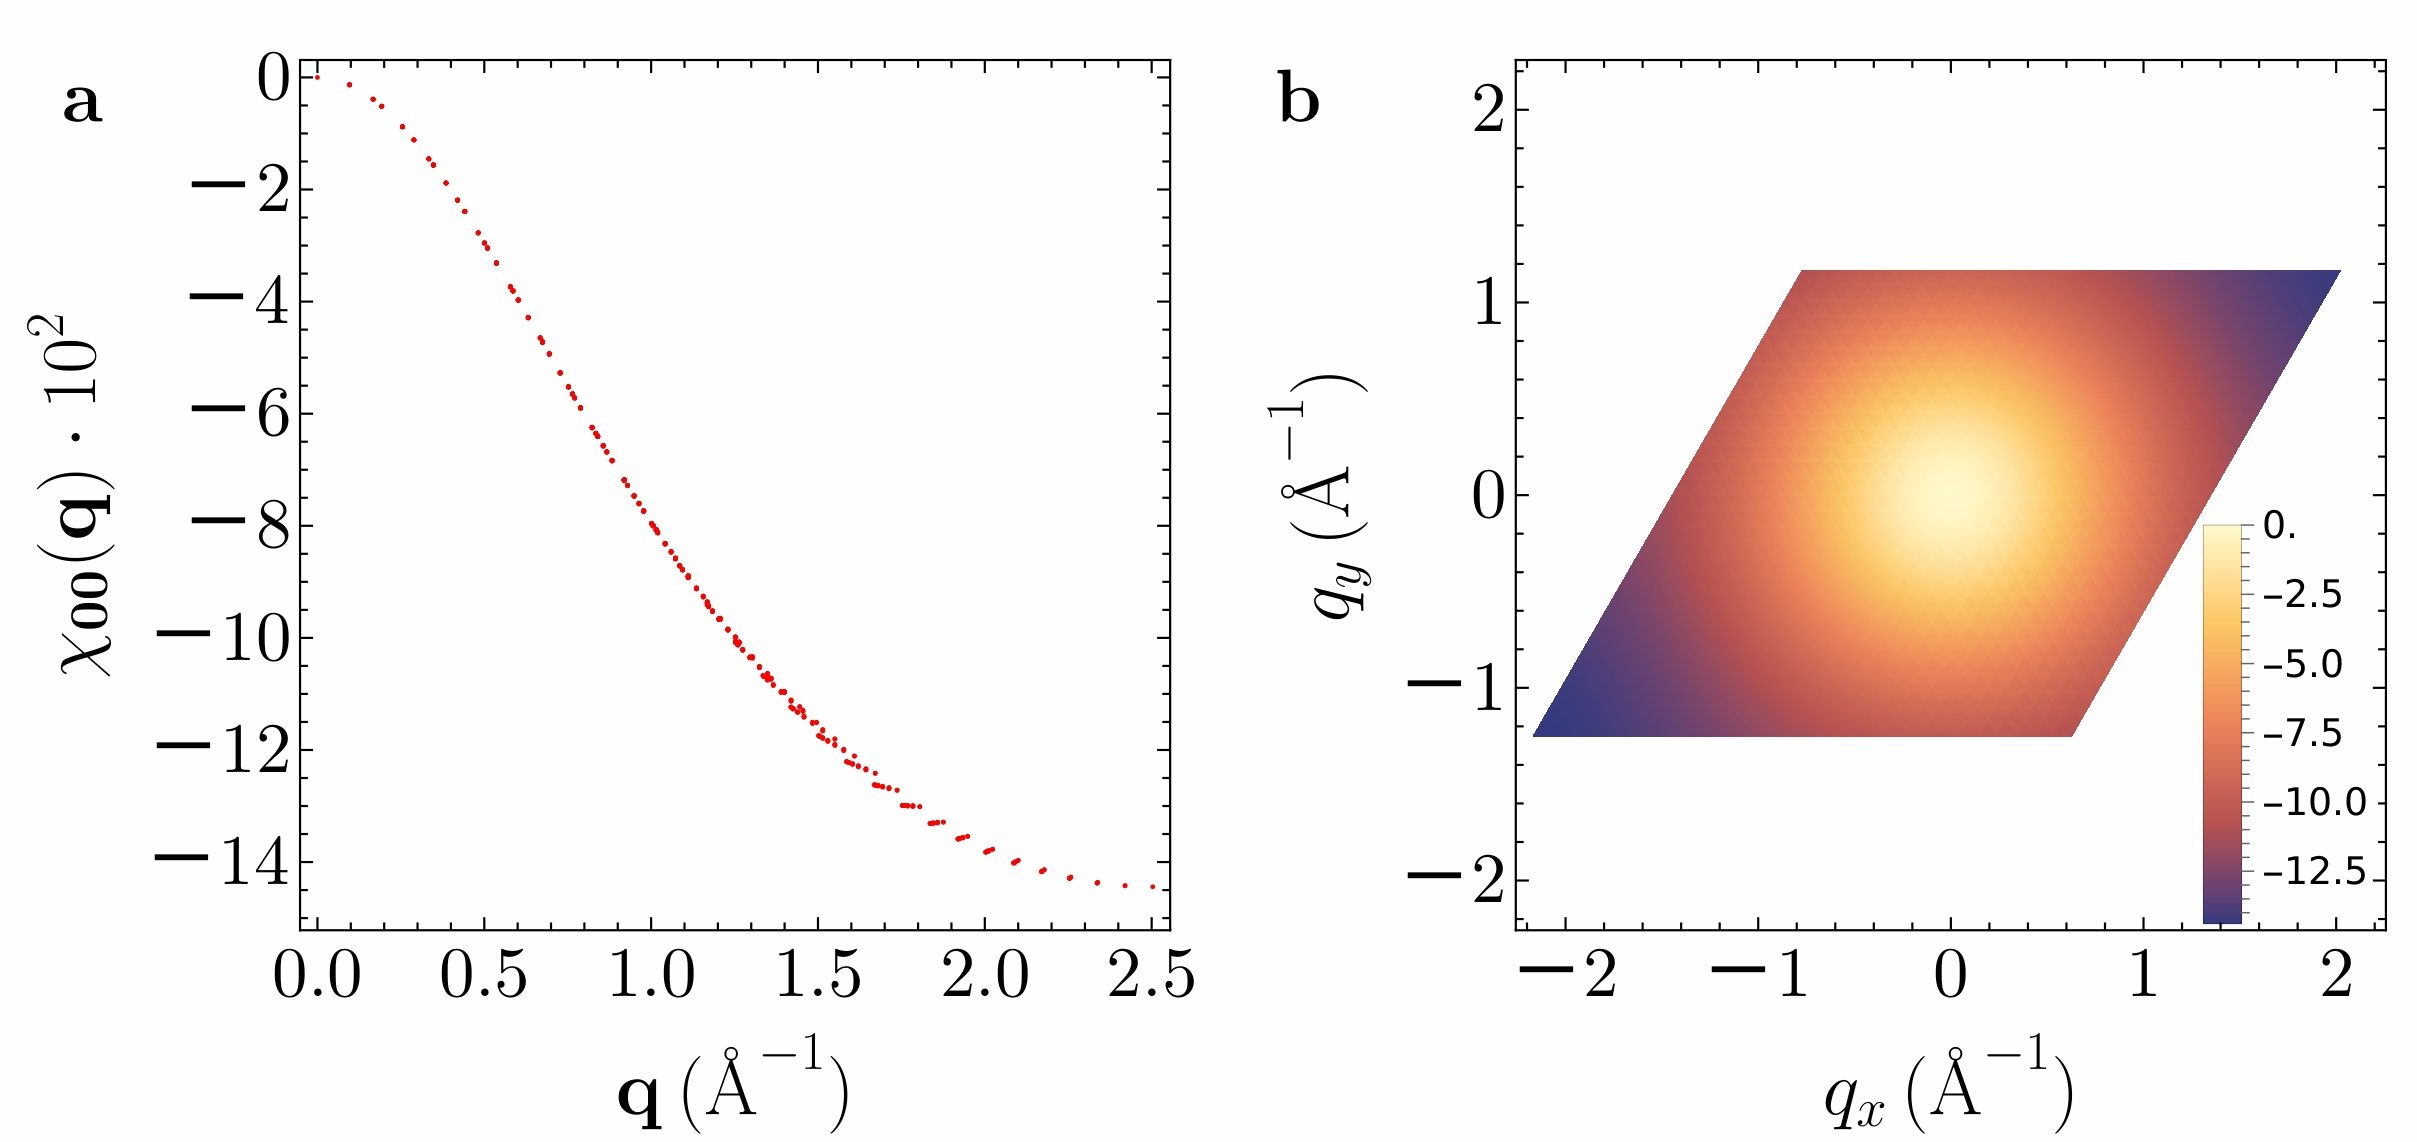
\includegraphics[width=1.0\textwidth]{Chapters/Figures/Chapter_6/Chi00hBNDFTmesh}
    \mycaption[Polarizability in the \bz~mesh: head element]{Matrix element $\chi^0_{\bzero \bzero} (\bq)$ of the polarizability in the \bz~for hBN, whose bands were obtained within \dft~ with the HSE06 functional. Panel \textbf{a} displays the polarizability as a function of the magnitude of the momentum along three directions: red dots include all the $\bq$ points in the mesh, blue dots correspond to the direction along the horizontal axis and dashed purple markers correspond to the direction parallel to the reciprocal lattice vector along the side of the parallelogram. Panel \textbf{b} displays a color map of the (absolute) value of the polarizability in the \bz~mesh. The bar legend for the colors is inside the plot.}
    \label{fig:chi_00_hbndft_mesh}
\end{figure}

\begin{figure}[H]
    \centering
    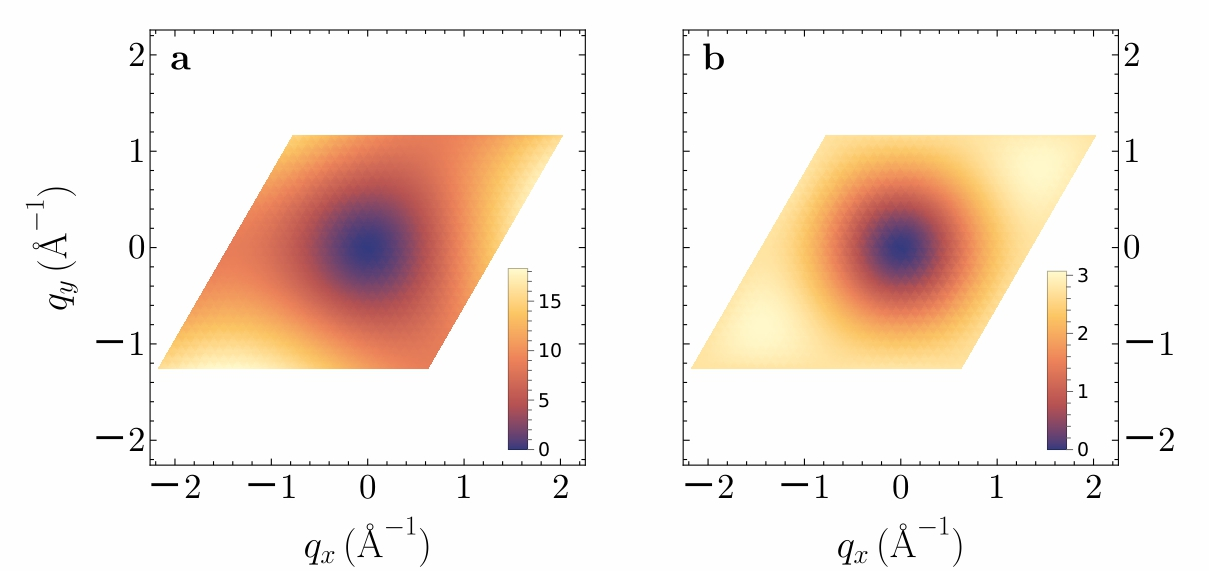
\includegraphics[width=1.0\textwidth]{Chapters/Figures/Chapter_6/ChiG1_0hBNDFTmesh}
    \mycaption[Polarizability in the \bz~mesh: an off-diagonal element]{Matrix element $\chi^0_{\bG_1 \bzero} (\bq)$ of the polarizability in the \bz~for hBN, whose bands were obtained within \dft~ with the HSE06 functional. Here $\bG_1 = \SIvector{-0.289052,0}{\angstrominverse}$. Panel \textbf{a} displays the real part of the polarizability, while panel \textbf{b} displays the imaginary part. The bar legend for the colors are inside the respective plots.}
    \label{fig:chi_g10_hbndft_mesh}
\end{figure}

As we now already have the polarizability, we can compute the matrix elements of the static dielectric function following Eq.~\eqref{eq:static_dielectric_function}.
In fact, we have implemented a symmetrized version of the dielectric function given by

\begin{empheq}[innerbox=\fbox, right={\,,}]{align}
    \label{eq:static_dielectric_function_symmetric}
    \varepsilon_{\bG \bG'} (\bq) = \delta_{\bG \bG'} - \sqrt{v_c(\bq + \bG)} \chi^0_{\bG \bG'} (\bq) \sqrt{v_c(\bq + \bG')}
\end{empheq}

\noindent for reasons that will become clear later on.
\todo{keep working on the figures in the notebook}


\subsection{Inverse dielectric matrix: convergence and the macroscopic dielectric function}
\label{subsec:inverse_dielectric_matrix_results}

\subsubsection{Local-field effects and convergence}
\label{subsubsec:inv_dielectric_matrix_convergence}

Here we study the convergence of the inverse dielectric matrix with the number of included reciprocal lattice vectors.
This is the most sensitive point---choosing an appropriate cutoff $G_c$ to compute the inverse dielectric matrix $\varepsilon^{-1}_{\bG \bG'} (\bq)$.
For the matrix elements to converge, we need a high enough number of reciprocal lattice vectors.
We compute the matrix $\varepsilon^{-1}_{\bG \bG'} (\bq)$ for $\bq \neq 0$ with an increasing number of reciprocal lattice vectors included, and inspect four matrix elements: the head element, two body elements, a diagonal one and an off-diagonal one, and a wing element.
A wing element is an element of the form $\varepsilon^{-1}_{\bG \bzero} (\bq)$ or $\varepsilon^{-1}_{\bzero \bG} (\bq)$ with $\bG \neq \bzero$, and a body element is an element of the form $\varepsilon^{-1}_{\bG \bG'} (\bq)$ with $\bG \neq \bzero$ and $\bG' \neq \bzero$.
In Fig.~\ref{fig:hBN_inv_epsilon_convergence} below we showcase four matrix elements of the inverse dielectric matrix, one in each panel.
For each point in each curve, we applied a cutoff $G_c$ in integer multiples of $3 \text{\unit{\angstrom}}^{-1}$, but the horizontal axis shows the number of vectors included, and not the cutoff.
We can notice a convergence tendency with the number of reciprocal lattice vectors, albeit quite slow.

\begin{figure}[H]
    \centering
    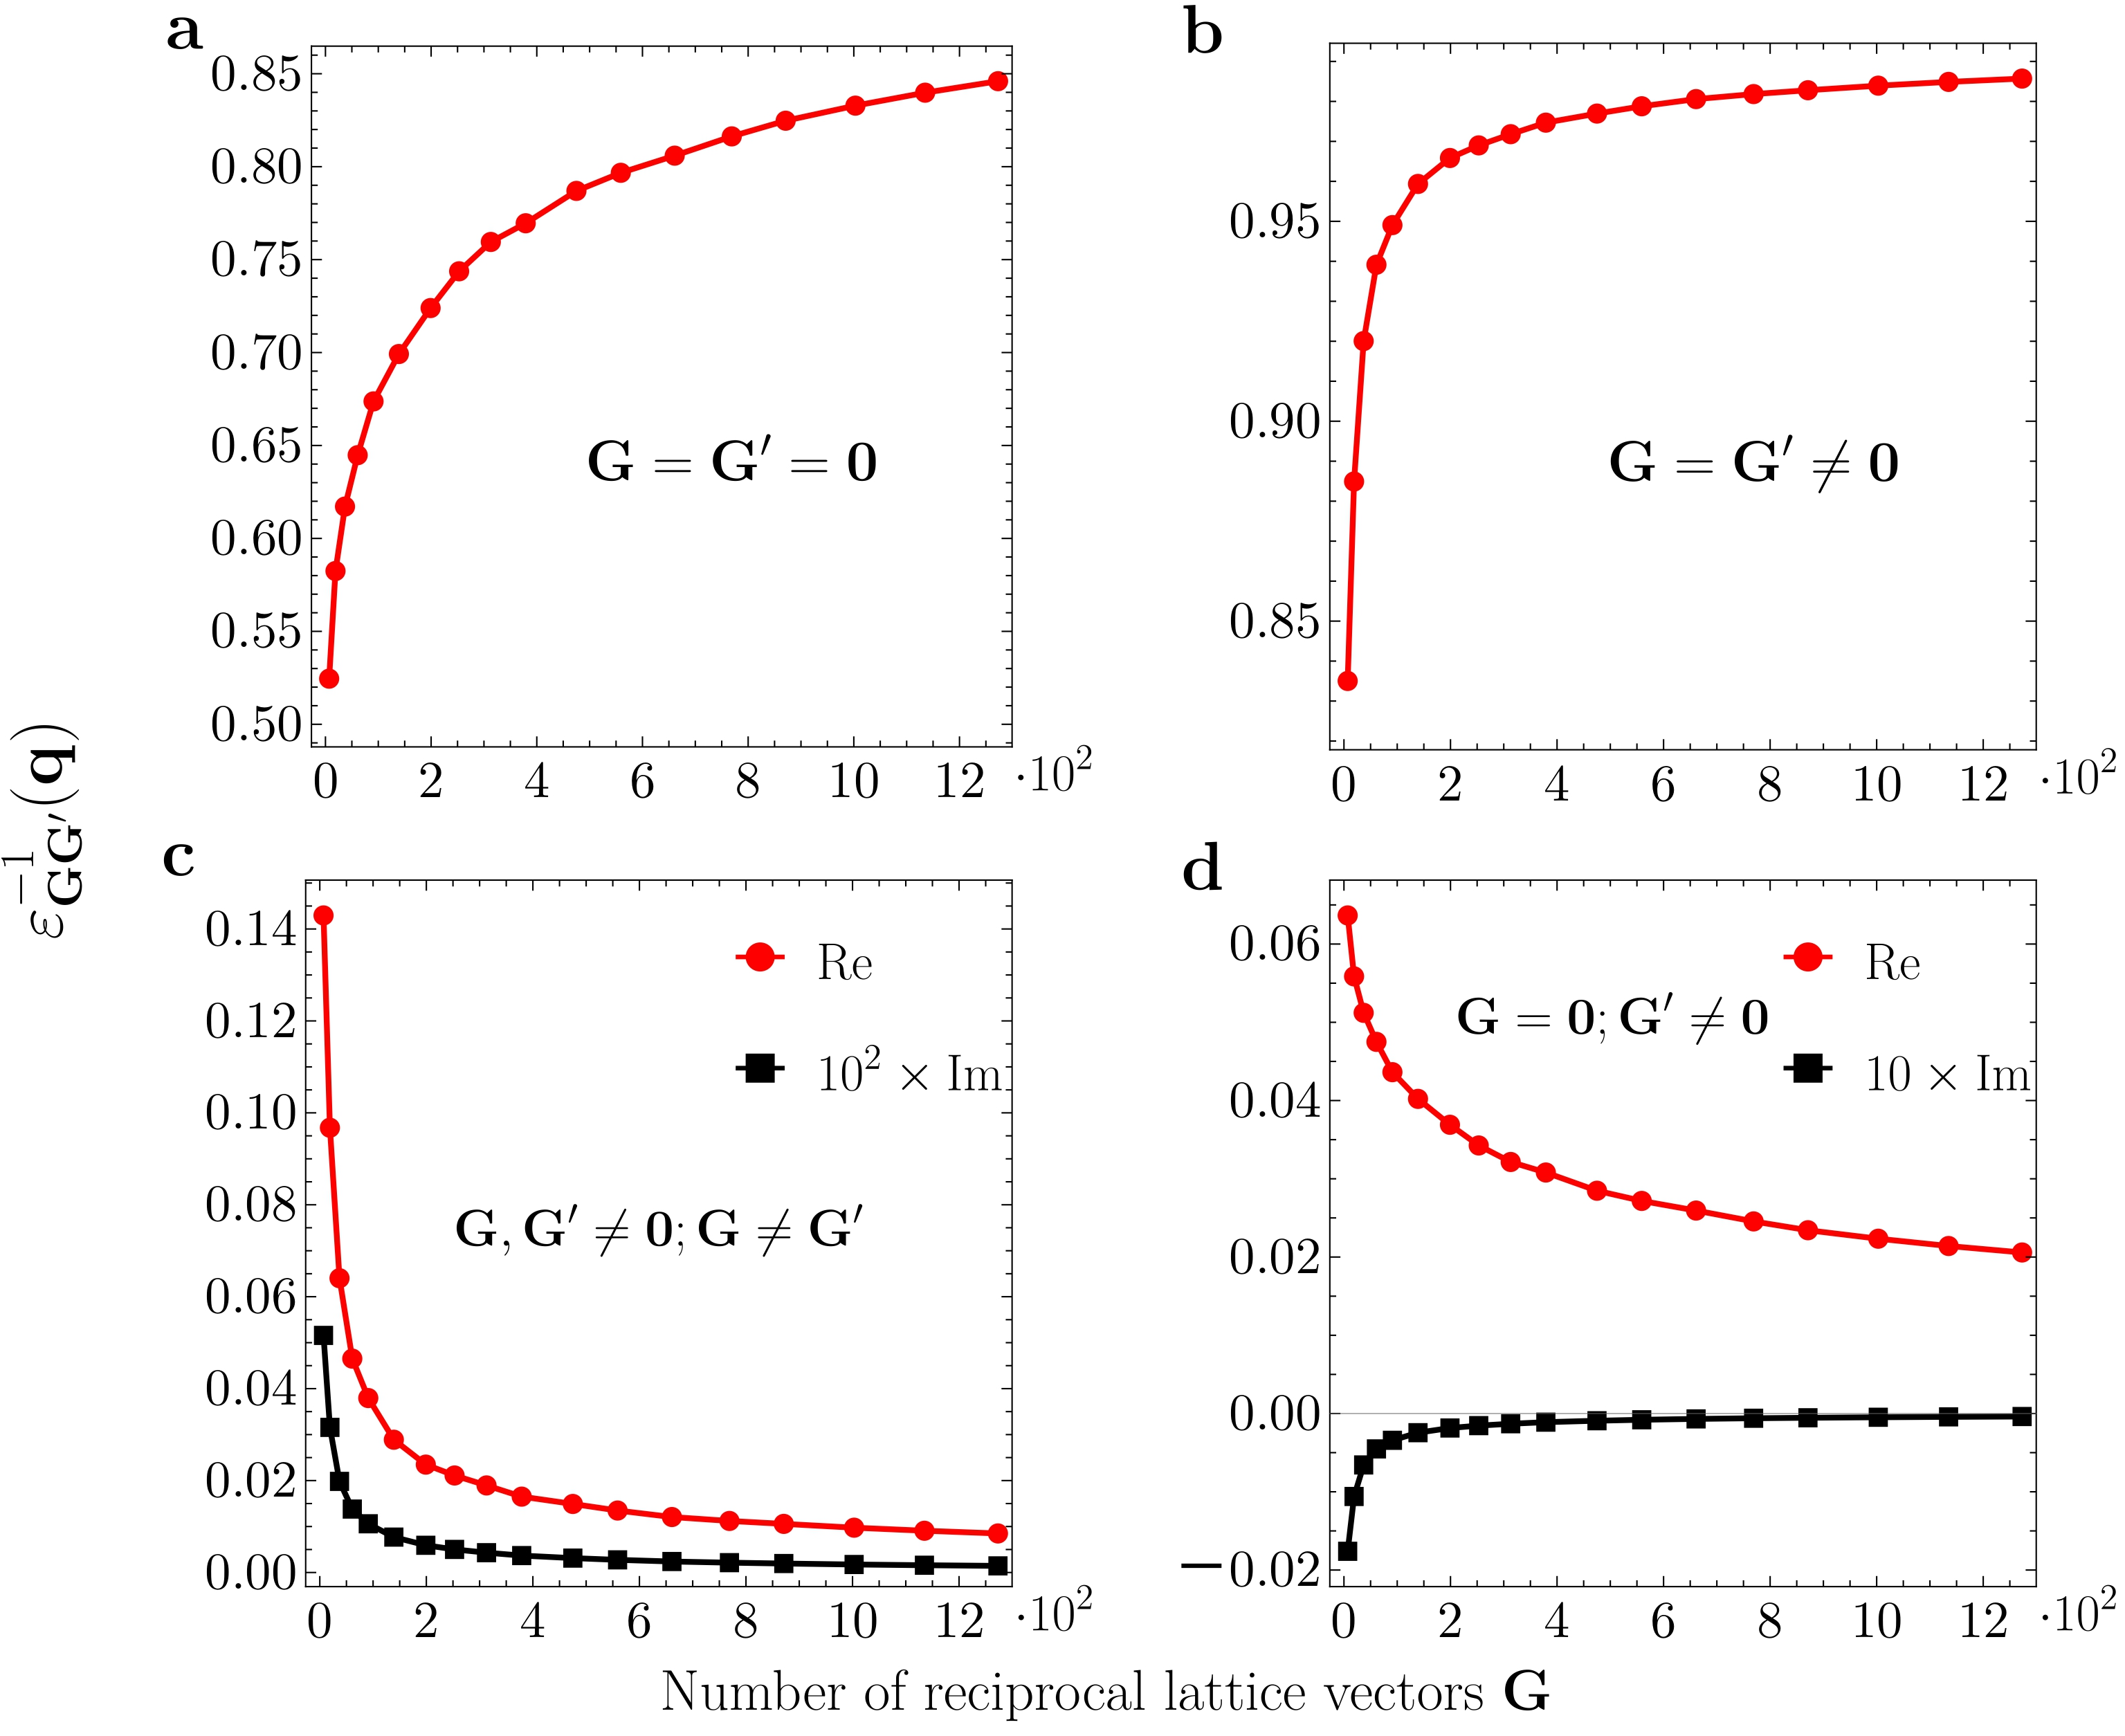
\includegraphics[width=1.0\textwidth]{Chapters/Figures/Chapter_6/inv_epsilon_convergence_hBN_panels}
    \mycaption[Convergence of the inverse dielectric matrix]{Selection of matrix elements $\varepsilon^{-1}_{\bG \bG'} (\bq)$ of the inverse of the dielectric matrix $\varepsilon^{-1}_{\bG \bG'} (\bq)$ computed at a point $\bq \neq \bzero$ in the \bz, for our model of \gls{hbn} from CRYSTAL.}
    \label{fig:hBN_inv_epsilon_convergence}
\end{figure}

\subsubsection{Macroscopic 2D dielectric function}
\label{subsubsec:macroscopic_dielectric_function}

Important to compare with ab initio results, and to recover Rytova-Keldysh potential.

\subsection{Excitonic states and conductivity}
\label{subsec:excitons_results}

Here goes what happened to the excitons with the new screening.
The numerical conductivity could also be used to recalculate the exciton-polaritons.

\subsection{Quasi-2D picture}
\label{subsec:quasi_2D}

\section{Efficient computation of the static dielectric function with the Xatu code}
\label{sec:xatu_code}

This is a section devoted solely to the code and implementation.
As a paper did not come out of the implementation at the time of submission, this chapter can probably be deemed secondary.
Also if I don't have the time to write it at the end, then I won't include it at all, or just make it very brief.